\section{O mercado de energia elétrica brasileira}


\subsection{Origens}

O Brasil, no início do setor elétrico, possuia quatro empresas estatais,
criadas pelo governo federal, para suprir as necessidades energéticas
da população. Cada uma operava numa região distinta: Norte (Eletronorte),
Nordeste (Chesf), Sul (Eletrosul) e Sudeste (Furnas). Eletrobrás coordenava
as quatro empresas. Atuavam fornecendo a energia. Cada sistema era
isolado do outro.

Marco histórico também foi o tratado de Itaipu, em 1973, que permitiu
a exploração do potencial hídrico do rio Paraná, pertencente ao Brasil
e ao Paraguai. Este tratado vigora até o ano de 2023.

A primeira empresa de distribuição criada no Brasil foi a Light. Inicialmente
fundada por um grupo canadense, até ser comprada pelo governo brasileiro,
no final da década de 1970. Na década de 1990, ela foi comprada do
governo por um grupo francês.

A primeira integração entre as regiões foi através da interligação
das regiões Sul com Sudeste e Norte com Nordeste. 

A operação era, em muitas vezes, deficitária. O governo via o investimento
na energia elétrica como algo prioritário para o desenvolvimento do
país. Na construção de usinas, muito emprego foi gerado, muitas construtoras
cresceram, e a população possuía energia para alçar voos mais altos.
Com o tempo e a necessidade de maior controle das operações, foram
criadas as empresas estaduais de energia, 

As únicas usinas que as empresas do setor privado poderiam produzir
eram para suprir sua própria demanda. Não era permitido que elas vendessem
energia para outros consumidores.Assim, neste período, o Brasil possuía
as empresas federais, cuidando de grande parte da produção, e algumas
ilhas de produção por parte de empresas privadas. 

As empresas tinham pouco incentivo para melhorias. O lucro de uma
empresa cobria o prejuízo das outras, já que o governo era o ``dono''
de todas. No final da década de 80, o Brasil se encontrava numa crise
econômica grave. O lucro das empresas elétricas, quando havia, era
utilizado para tapar buracos para outras necessidades do governo brasileiro.
Assim, no final de 1993, o setor entrou em crise grave, com a maioria
das obras paradas de construção de usinas paradas. Esta crise motivou
uma reforma geral no setor elétrico, já que o governo não possuia
mais dinheiro para investir na sua expansão.

\begin{figure}
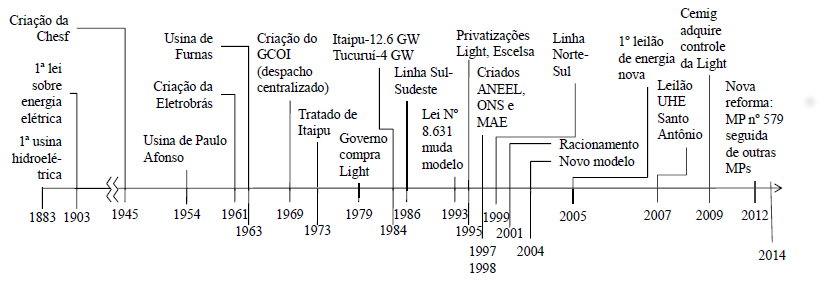
\includegraphics[scale=0.75]{anexos/aula11_1}

\protect\caption{Linha do tempo do setor no Brasil \label{fig:Linha-do-tempo}}
\end{figure}


A Lei 8.631 permitiu que as concessionárias ajustassem seus preços
de serviço. Além disso, essa lei permitiu a criação de duas tarifas
distintas: uma para a geração e outra para a distribuição da energia.

Neste momento, ocorria a descentralização das atividades do setor
elétrico. Enquanto antes todas as etapas eram feitas pela mesma empresa,
agora a cadeia produtiva estava sendo dividida em geração, transmissão,
distribuição e comecialização da energia.

Privatização do setor. Vender as empresas com intuito de arrecadação.
Assim, as usinas de energia, que forneceriam para os consumidores,
passam a ficar nas mãos da iniciativa privada. Foi necessário criar,
portanto, uma agência reguladora para o mercado que estava nascendo:
a ANEEL. 

A Eletrobrás, que até então detinha a tarefa de operadora do sistema,
não podia mais exercê-la, já que agora era uma das várias empresas
que competiam no mercado de energia. Assim como não se deixa o lobo
tomando conta do galinheiro, esta função teria que sair da Eletrobrás.
Para isso, foi criada a ONS.

O MAE é o mercado atacadista de energia. A função deste mercado é
basicamente fornecer o meio para a liquidação dos contratos de energia.

A privatização começou pela distribuição. A razão para isso é que,
para que empresas viessem se instalar para a geração, era necessário
criar uma boa capacidade de pagamento, e garantir que quem gerasse
energia tivesse confiança que havia crédito. O setor privado, portanto,
traria capital a mais para setor. Ao mesmo tempo, as distribuidoras
estavam sem dinheiro no Brasil. Essa estratégia de começar as privatizações
pelas empresas distribuidoras foi adotada não apenas pelo Brasil,
mas também por Argentina, Turquia, Colômbia, entre outros. Neste processo,
75\% das empresas foram privatizadas.

O sistema ficou, portanto, com gande proporção de empresas privadas
na distribuição, e maioria de empresas públicas na geração. Para que
este mixto entre público e privado funcione no mercado, é necessário
que as empresas públicas sejam orientadas para o lucro, ou seja, serem
economicamente racionais. Muitas vezes, isso não é ocorre, pois os
governos se utilizam das empresas públicas para fazerem políticas
sociais.

Em 1995, vieram as leis de Concessão (Lei 8.987/95 e 9.074/95), cujo
objetivo era regulamentar os direitos e deveres de uma empresa que
se utiliza de um bem público: no caso, a água. Essa lei outorgou a
concessão por 20 anos. A possibilidade de fazer investimentos em pequenos
usinas foi o grande chamariz para que o setor privado entrasse de
vez no setor elétrico. Já a transmissão e a distribuição, que são
atividades caracterizadas como de monopólio natural, quando liberadas
para empresas privadas devem ser reguladas.

Há uma diferença crucial entre um investidor querer entrar no mercado
construindo uma hidrelétrica ou construindo um outro tipo de usina:
a hidrelétrica se utiliza de um bem público para funcionar, enquanto
uma outra, como por exemplo uma termelétrica, não. Assim, para construir
uma termelétrica, bastava pedir uma autorização ao governo.

Quem quisesse entrar no mercado com uma usina hidrelética, no entanto,
teria que tomar outro caminho. O governo tomou a iniciativa de realizar
leilões de projetos hidrelétricos, em que ganhava aquela empresa que
fornecesse a maior mesada para assumir aquela concessão pelo prazo
de, por exemplo, 30 anos. 

\begin{figure}
\begin{centering}
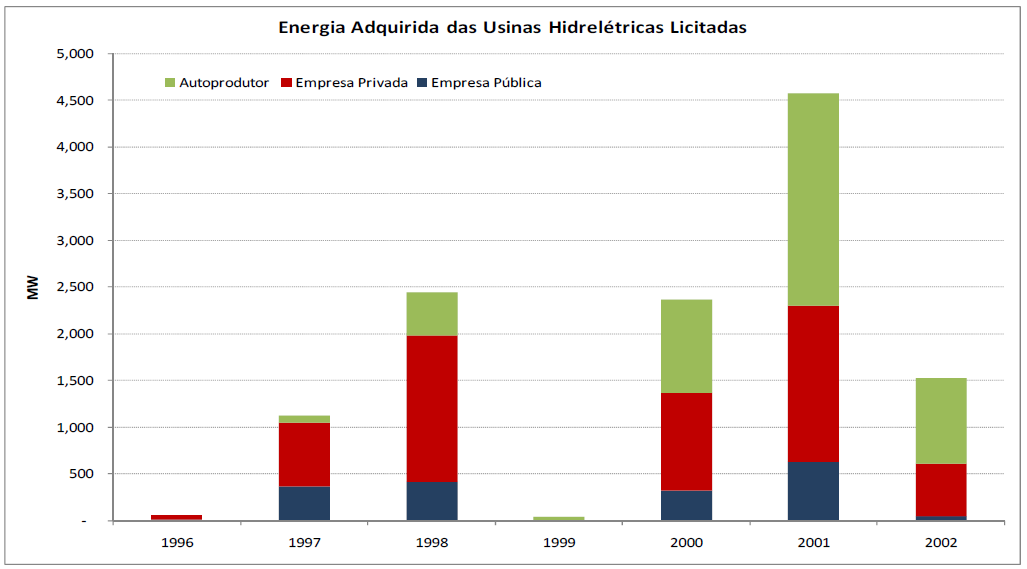
\includegraphics[scale=0.5]{anexos/aula110-1}
\par\end{centering}

\protect\caption{}


\end{figure}


A decisão da construção de uma linha de transmissão é definido pelas
agências reguladoras, através de uma decisão unilateral. Depois de
decidir as linhas que devem ser construídas, é feito um leilão em
que as empresas interessadas expõe seus preços para a construção da
linha e para mantê-la disponível para transmissão. 

A tarifa pela utilização da linha de transmissão se dá de acordo com
a localização da usina acessante. O potencial de privarização é limitado;
no entanto, as licitação da transmissão são bem-sucedidas.


\subsubsection*{Racionamento}

No final da década de 1990, houve uma diminuição do nível dos reservatórios,
devido a um período de baixas chuvas. A figura \ref{fig:nivel-reserv}
mostra a queda no nível de reservatório com o passar dos anos. Em
março de 2011, a situação já estava num nível emergencial. A solução
adotada pelo governo foi mergulhar o país num racionamento de energia.
O objetivo era diminuir consideravelmente a demanda por energia para
que os reservatórios pudessem voltar a um nível adequado. O racionamento
foi decretado em maio de 2011, abrangendo as regiões Norte, Nordeste,
Sudeste e Centro-Oeste. Com essa política, a demanda por energia foi
reduzida em 20\%.

\begin{figure}
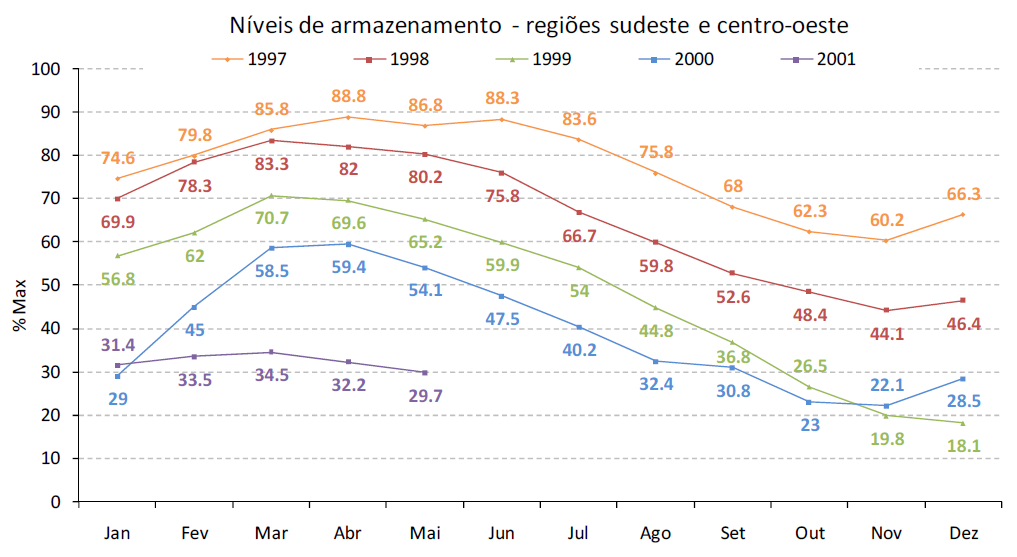
\includegraphics[scale=0.5]{anexos/aula110-2}

\protect\caption{\label{fig:nivel-reserv}}
\end{figure}


Depois da crise, um novo modelo era necessário. A seção seguinte descreve
brevemente a estrutura das agências reguladoras .


\subsection{Insituições reguladoras}

Preço no mercado: vem do custo marginal de produção. Apenas as grandes
indústrias teriam acesso ao mercado livre de energia. Os consumidores
de pequeno porte, como pessoas físicas, apenas podem contratar energia
da distribuidora (forma como é até hoje).

ANP: Enquanto no mundo inteiro a agência que regula a energia elétrica
é a mesma que regula óleo e gás, no brasil há uma instituição específica
para regular eles.

\begin{table}
\begin{tabular}{>{\raggedright}p{0.3\textwidth}|>{\raggedright}p{0.6\textwidth}}
\hline 
Agentes & Funções\tabularnewline
\hline 
\hline 
Conselho Nacional de Política Energética - CNPE & Homologação da política energética, em articulação com as demais políticas
públicas\tabularnewline
\hline 
Ministério de Minas e Energia - MME & Formulação de políticas para o setor energético; implementação dessas
políticas energéticas; e exercício do poder concedente\tabularnewline
\hline 
Agência Nacional de Energia Elétrica - ANEEL & Mediação, regulação e fiscalização do funcionamento do sistema elétrico,
envolvendo o cumprimento das normas do marco regulatório em geral
e das obrigações dispostas nos atos de outorga (contratos de concessão,
autorização ou permissão) dos serviços de geração, transmissão e distribuição\tabularnewline
\hline 
Empresa de Pesquisa Energética - EPE & Execução dos estudos de planejamento energético\tabularnewline
\hline 
Câmara de Comercialização de Energia Elétrica - CCEE & Contabilização e liquidação de diferenças contratuais no curto prazo;
e administração dos contratos de compra de energia para atendimento
aos consumidores regulados\tabularnewline
\hline 
Operador Nacional do Sistema Elétrico - ONS & Operação integrada e centralizada do sistema elétrico interligado;
e administração da contratação das instalações de transmissão\tabularnewline
\hline 
Operador dos Sistemas Elétricos Isolados & Coordenação da operação dos sistemas elétricos isolados\tabularnewline
\hline 
Comitê de Monitoramento do Setor Elétrico - CMSE & Monitoramento das condições de atendimento, no horizonte de cinco
anos, com o objetivo de assegurar a implementação de providências
com vistas a garantir a normalidade do suprimento de energia elétrica
(coordenação do MME, com apoio da EPE, CCEE, da ANEEL e do ONS)\tabularnewline
\hline 
Eletrobrás & Financiamento, em caráter suplementar, da expansão do setor elétrico;
exercício da função de holding das empresas estatais federais; administração
de encargos e fundos setoriais; comercialização da energia de Itaipu
e de fontes alternativas contempladas pelo PROINFA; e Coordenação
do OSI\tabularnewline
\hline 
\end{tabular}

Fonte: \ref{landi2006energia}

\protect\caption{Principais agentes e suas funções\label{tab:instituicoes}}
\end{table}


A ONS despacha centralizadamente o sistema através de modelos computacionais
e calculam os custos de oportunidade das usinas hidrelétricas. A determinação
dos preços do mercado são pelo custo marginal de operação, que é a
base para formar o Preço de Liquidação de Diferenças (PLD) na CCEE.
O PLD é o \textquotedblleft preço de curto prazo\textquotedblright{}
da energia no Brasil, que remunera todos os geradores em um \textquotedblleft mercado
atacadista. 

Assim, a função do PLD é fornecer um sinal para a expansão do sistema.
Por exemplo, se há poucas usinas fornecendo energia, o preço de liquidação
será alto, pois há escassez de oferta no mercado. Uma dificuldade
prática na implantação do esquema \textquotedblleft puro\textquotedblright{}
de mercado no Brasil é a variabilidade dos preços da energia, pois
ele introduz incertezas na remuneração dos geradores e dificulta sua
viabilidade comercial e financiabilidade.

Para combater o problema da variabilidade do preço do PLD, as empresas
comercializadores de energia que desejem vender uma certa quantidade
de energia, devem possuir contratos suficientes para suprir a energia
em contrato. Os contratos de suprimento estão no núcleo das negociações
de energia no Brasil (gerência de risco). Todo consumo deve estar
100\% contratadoA forma de negociar os contratos é o que diferencia
o \textquotedblleft mercado livre\textquotedblright{} do mercado regulado\textquotedblright . 

O ambiente de contratação regulada (ACR) é aquele regime no qual as
distribuidoras (75\% do mercado) contratam energia. Elas o fazem somente
através de leilões de contratos: processo organizado de leilões de
contratos para distintas finalidades. Já o ambiente de contratação
livre (ACL) é um ambiente para consumidores livres (25\% do mercado)
se contratam como quiserem, desde que estejam 100\% contratados. Apenas
consumidores de grande porte podem comprar energia nesse mercado.
É feita uma verificação ex-post mensal se a integral do consumo nos
últimos 12 meses está coberta por contratos de compra. Se houver subcontratação,
uma multa é aplicada às empresas que oferecem os contratos de energia. 

A exigência de contratação do mercado de energia tem como objetivo
principal a segurança do sistema. Com isso, impede-se que companhias
tentem arbitrar a todo custo, com prejuízos eventuais ao consumidor
quando esta vende energia mas na hora de entregar não possuí-la.

É necessário, no entanto, uma metodologia para definir quanto de energia
uma dada usina consegue fornecer. Essa quantidade é denominada \textbf{garantia
física de um equipamento} e mede sua contribuição energética para
a confiabilidade de suprimento. Atribuída em MWh/ano, possui duas
importâncias: (i) Física: segurança de suprimento; (ii) Comercial:
é a maior quantidade de energia que um projeto pode comercializar
em contratos de suprimento de energia e é a cota de participação no
MRE. A garantia física é calculada pela EPE e, de forma simplificada,
é a maior quantidade de energia que ele pode entregar dado um critério
de confiabilidade (ocorrência de um ano seco): critérios definidos
na Portaria 258/2008 do MME.

A confiabilidade de suprimento é uma propriedade sistêmica (\textquotedblleft bem
comum\textquotedblright ) e há uma sinergia entre as confiabilidades
individual (cada projeto) e sistêmica. Como os perfis de geração podem
ser diferentes entre diferentes sistemas, temos que:

\[
\mbox{Confiabilidade}(A+B)\geq\mbox{confiabilidade}(A)+\mbox{confiabilidade}(B).
\]
O cálculo da garantia física é realizado em duas etapas: 
\begin{enumerate}
\item Cálculo da garantia física total do sistema de acordo com o critério
de suprimento.
\item Rateio da garantia física total entre as usinas individuais. 
\end{enumerate}
O critério de suprimento e de rateio são definidos na Portaria 258/2008
do MME.

Simplificadamente, a garantia física de uma hidroelétrica é proporcional
à sua produção na pior seca observada no registro histórico de vazões.
Para termoelétricas, a garantia física também é proporcional à sua
contribuição nos períodos secos. O que \textquotedblleft conta\textquotedblright{}
não é a capacidade de produção em um momento específico mas a produção
observada ao longo de um período seco. A contribuição de energia das
térmicas depende do seu acionamento no período crítico, dependendo
portanto do seu custo variável unitário e de sua inflexibilidade.
A figura \ref{fig:Exemplos-da-rela=0000E7=0000E3o-1} mostra a relação
da garantia física com o custo operativa e a inflexibilidade da usina,
enquanto a figura \ref{fig:Esquema-dos-passos} mostra um esquema
do processo de definição da garantia física.

\begin{figure}
\begin{centering}
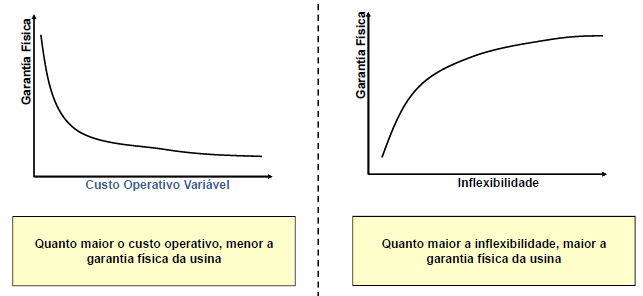
\includegraphics{anexos/aula110-4}
\par\end{centering}

\protect\caption{Exemplos da relação entre parâmetro informado e garantia física resultante\label{fig:Exemplos-da-rela=0000E7=0000E3o-1}}
\end{figure}


\begin{figure}
\begin{centering}
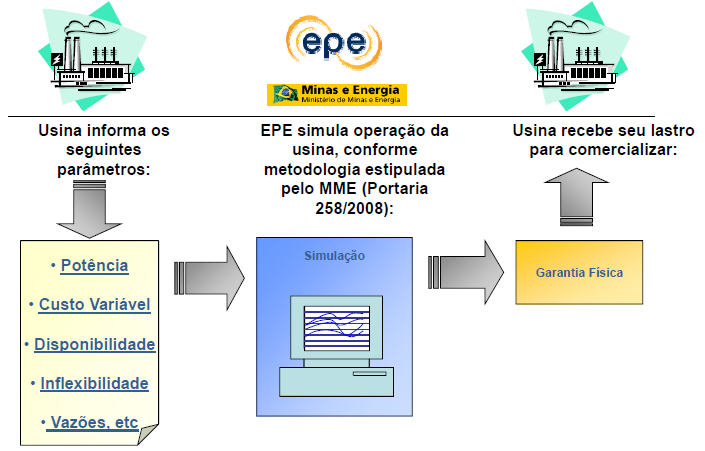
\includegraphics[scale=0.8]{anexos/aula110-5}
\par\end{centering}

\protect\caption{Esquema dos passos para a definição da garantia física de uma usina\label{fig:Esquema-dos-passos}}
\end{figure}


A figura \ref{fig:Gera=0000E7=0000E3o-f=0000EDsica-vs.} mostra como
a geração física num determinado momento é diferente da energia assegurada,
ou seja, há muita variabilidade na geração das hidrelétrica, por causa
da sazonalidade da época de chuvas. Para melhor a quantidade de energia
a ser fornecida de forma estável, foi criado o Mecanismo de Realocação
de Energia (MRE). 

O MRE é um \textquotedblleft condomínio\textquotedblright{} fictício
onde cada participante (usina hidro) tem uma determinada quantidade
de \textquotedblleft cotas\textquotedblright{} Energia Alocada (MWh).
Este condomínio recolhe a soma dos recebimentos na CCEE de todos os
MRE participantes. O montante total recolhido é então distribuído
entre os participantes em proporção à suas \textquotedblleft cotas\textquotedblright .
A figura \ref{fig:Quando-somadas} mostra o perfil de um MRE formado
por hidros com perfis de geração complementares, e como a energia
assegurada é muito maior que a soma das energias asseguradas individuais.
A cota de participação de cada usina no MRE é a sua garantia física.
A fração que cada gerador recebe do MRE é dada pela razão entre sua
cota e a soma das cotas de todos os participantes: 
\[
\dfrac{\mbox{Garantia física}}{\sum\mbox{garantia física do sistema}}
\]
No entanto, para efeitos de cálculo da energia alocada no MRE, a garantia
física pode ser reduzida se o fator de disponibilidade real da usina,
apurado pelo ONS, for inferior ao de referência. Para efeitos de cota
no MRE e lastro contratual, a garantia física pode variar mensalmente.

A fração que cada gerador recebe do MRE é dada pela razão entre sua
cota e a soma das cotas de todos os participantes. Esta fração pode
variar mensalmente: ano participantes poderiam declarar 12 valores
mensais para suas cotas de maneira Sazonalização arbitrária; a única
restrição é que a média das cotas declaradas seja igual à cota MWh
original. Assim, permite-se que um gerador ajuste melhor seu perfil
de recebimento das cotas a um contrato de suprimento. Isso é conhecido
como \textquotedblleft sazonalização do MRE\textquotedblright .

\begin{figure}
\centering{}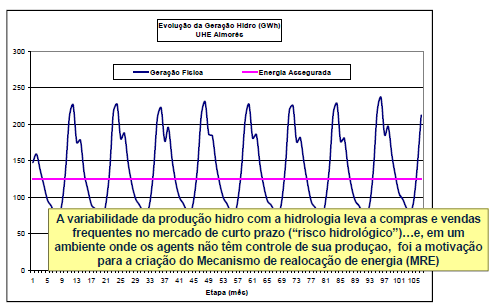
\includegraphics{anexos/aula110-6}\protect\caption{Geração física vs. Energia Assegurada\label{fig:Gera=0000E7=0000E3o-f=0000EDsica-vs.}}
\end{figure}


A obrigação de respaldo físico nos contratos de compra e venda de
energia significa que dois produtos estão sendo negociados. O primeiro
é a entrega de energia ao cliente (seja fisicamente ou financeiramente).
Em segundo, o lastro que respaldará o consumo do cliente.

\begin{figure}
\begin{centering}
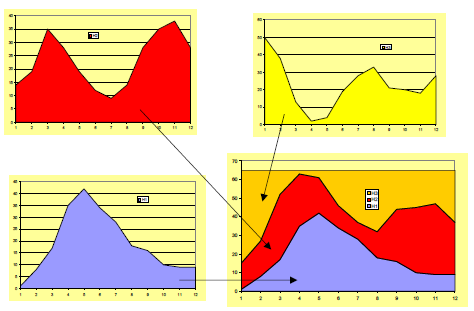
\includegraphics{anexos/aula110-7}
\par\end{centering}

\protect\caption{Quando somadas, as gerações das hidroelétricas possuem um perfil mais
estável\label{fig:Quando-somadas}}
\end{figure}


\begin{figure}
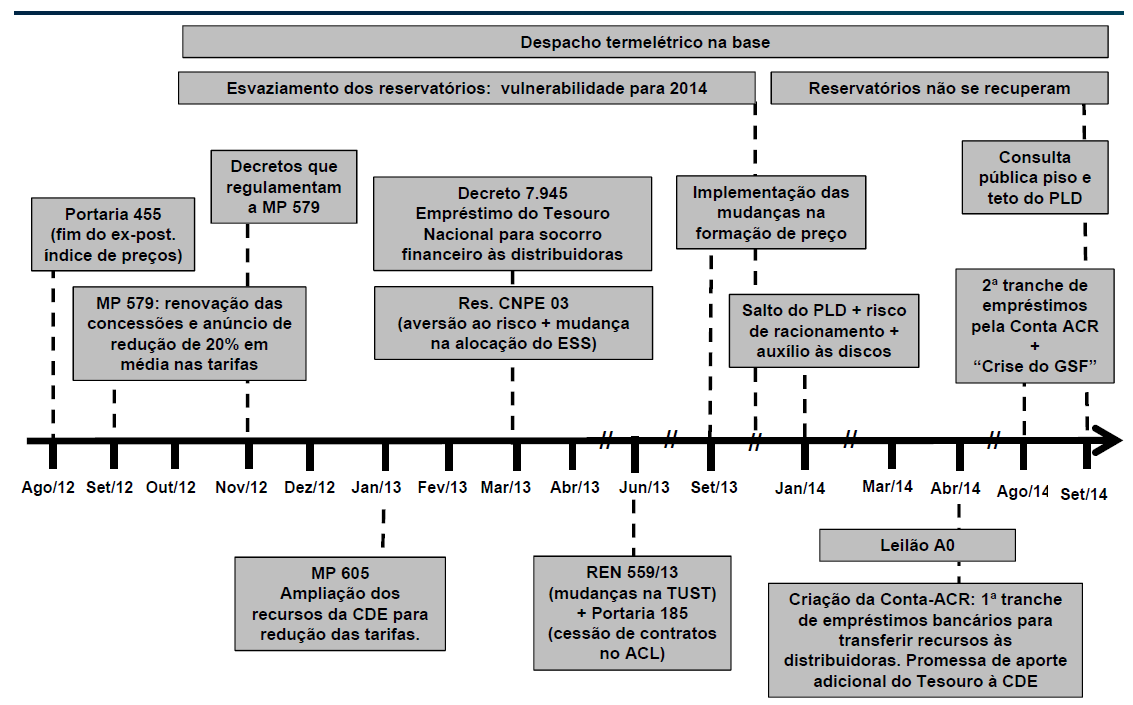
\includegraphics[scale=0.5]{anexos/aula110-}\protect\caption{Ambiente regulatório a partir de 2012 \label{fig:Ambiente-regulat=0000F3rio-a}}
\end{figure}


A tabela \ref{tab:instituicoes} mostra as instituições que cuidam
do mercado de energia brasileiro.

As concessões de geração e transmissão que venceriam em 2015 eram
uma grande oportunidade de reduzir as tarifas de energia. A forma
e montante da redução já eram debatidos por agentes do Setor desde
2008. Em setembro de 2012, foi publicada a Medida Provisória nº 579,
que estabeleceu mecanismos para renovar as concessões. O objetivo
era ambicioso: provocar redução de 20\% nas tarifas já em 2013. Para
isso, era preciso que todos os concessionários aderissem à proposta
de renovação antecipada das concessões (só parte dos geradores aderiu).
Assim, as reduções foram desequilibradas, favorecendo o mercado cativo;
elas dependiam de custos para a energia renovada que não se concretizaram,
e reduções significativas em despesas (ex. subsídio CCC) que também
não ocorreram. Elas tinham inicialmente como base os preços que deveriam
viger em 2013, os quais continham aumentos já \textquotedblleft contratados\textquotedblright{}
(ex. Angra) e seriam afetados pela situação do sistema. Além disso,
houve decisão de reduzir as tarifas nominais em 20\%. 

Como resultado dessas medidas houve um grande aperto e uma série de
correções de rumo. O Setor perdeu sua autossuficiência financeira.
Já foram publicadas 9 MPs e 9 decretos sobre Setor Elétrico desde
setembro de 2012 (ver figura \ref{fig:Ambiente-regulat=0000F3rio-a})
e a crise no setor continua presente em 2015.

O modelo atual guarda elementos que foram sendo agregados ao longo
do tempo. Do modelo \textquotedblleft antigo\textquotedblright , temos
várias empresas estatais, hoje em dia bem mais federais (boa parte
das distribuidoras que não foram privatizadas foi absorvida pela Eletrobrás).
Do modelo dos anos 90, temos a ANEEL, o ONS, distribuidores e geradores
privados, e os leilões de transmissão. Da revitalização, temos os
conceitos de segurança de suprimento através de contratação com respaldo
e leilões para suprimento a distribuidoras. Do modelo de 2004, temos
os leilões e a CCEE. Do modelo de 2012, temos as cotas de energia
resultantes das concessões e a volta do Tesouro ao Setor.

O modelo setorial parcialmente implantado nos anos 90 teve mantidas
algumas características básicas: competição na geração e na comercialização
aos consumidores livres, monopólios regulados na transmissão e na
distribuição e a presença de instituições específicas para regulação,
operação e relações comerciais. O modelo sofreu três reorientações
desde então. Em 2001, medidas emergenciais para conter a crise e ênfase
na contratação e no respaldo de garantia física. Em 2004, ênfase nos
leilões, na contratação e no respaldo de garantia física. Em 2012,
ênfase na redução das tarifas e medidas emergenciais para conter a
crise. O recente acúmulo de dívidas e aportes do Tesouro sugerem que
ciclo de revisão do modelo setorial ainda não foi concluído.
